\documentclass[11pt]{article}
\usepackage[textwidth=18.0cm, textheight=23.0cm, top=2.0cm]{geometry}
\usepackage{pst-all}
\usepackage{amssymb}
\usepackage{tikz}
\usepackage{underscore}\begin{document}
\pagestyle{empty}


ClassName: \underline{\textbf{Class_04.2bp-11}}
\par
BinSize: \underline{\textbf{100 × 100}}
\par
ReduceSize: \underline{\textbf{100 × 100}}
\par
TypeNum: \underline{\textbf{40}}
\par
Num: \underline{\textbf{40}}
\par
OutS: \underline{\textbf{20000}}
\par
InS: \underline{\textbf{11400}}
\par
Rate: \underline{\textbf{0.570}}
\par
UB: \underline{\textbf{2}}
\par
LB0: \underline{\textbf{2}}
\par
LB: \underline{\textbf{2}}
\par
LBWithCut: \underline{\textbf{2}}
\par
NodeCut: \underline{\textbf{0}}
\par
ExtendedNodeCnt: \underline{\textbf{1}}
\par
GenNodeCnt: \underline{\textbf{1}}
\par
PrimalNode: \underline{\textbf{0}}
\par
ColumnCount: \underline{\textbf{2}}
\par
TotalCutCount: \underline{\textbf{0}}
\par
RootCutCount: \underline{\textbf{0}}
\par
LPSolverCnt: \underline{\textbf{1}}
\par
PricingSolverCnt: \underline{\textbf{0}}
\par
BranchAndBoundNum: \underline{\textbf{1}}
\par
isOpt: \underline{\textbf{true}}
\par
TimeOnInitSolution: \underline{\textbf{0.000 s}}
\par
TimeOnPrimal: \underline{\textbf{0.000 s}}
\par
TimeOnPricing: \underline{\textbf{0.000 s}}
\par
TimeOnRmp: \underline{\textbf{0.062 s}}
\par
TotalTime: \underline{\textbf{0.125 s}}
\par
\newpage


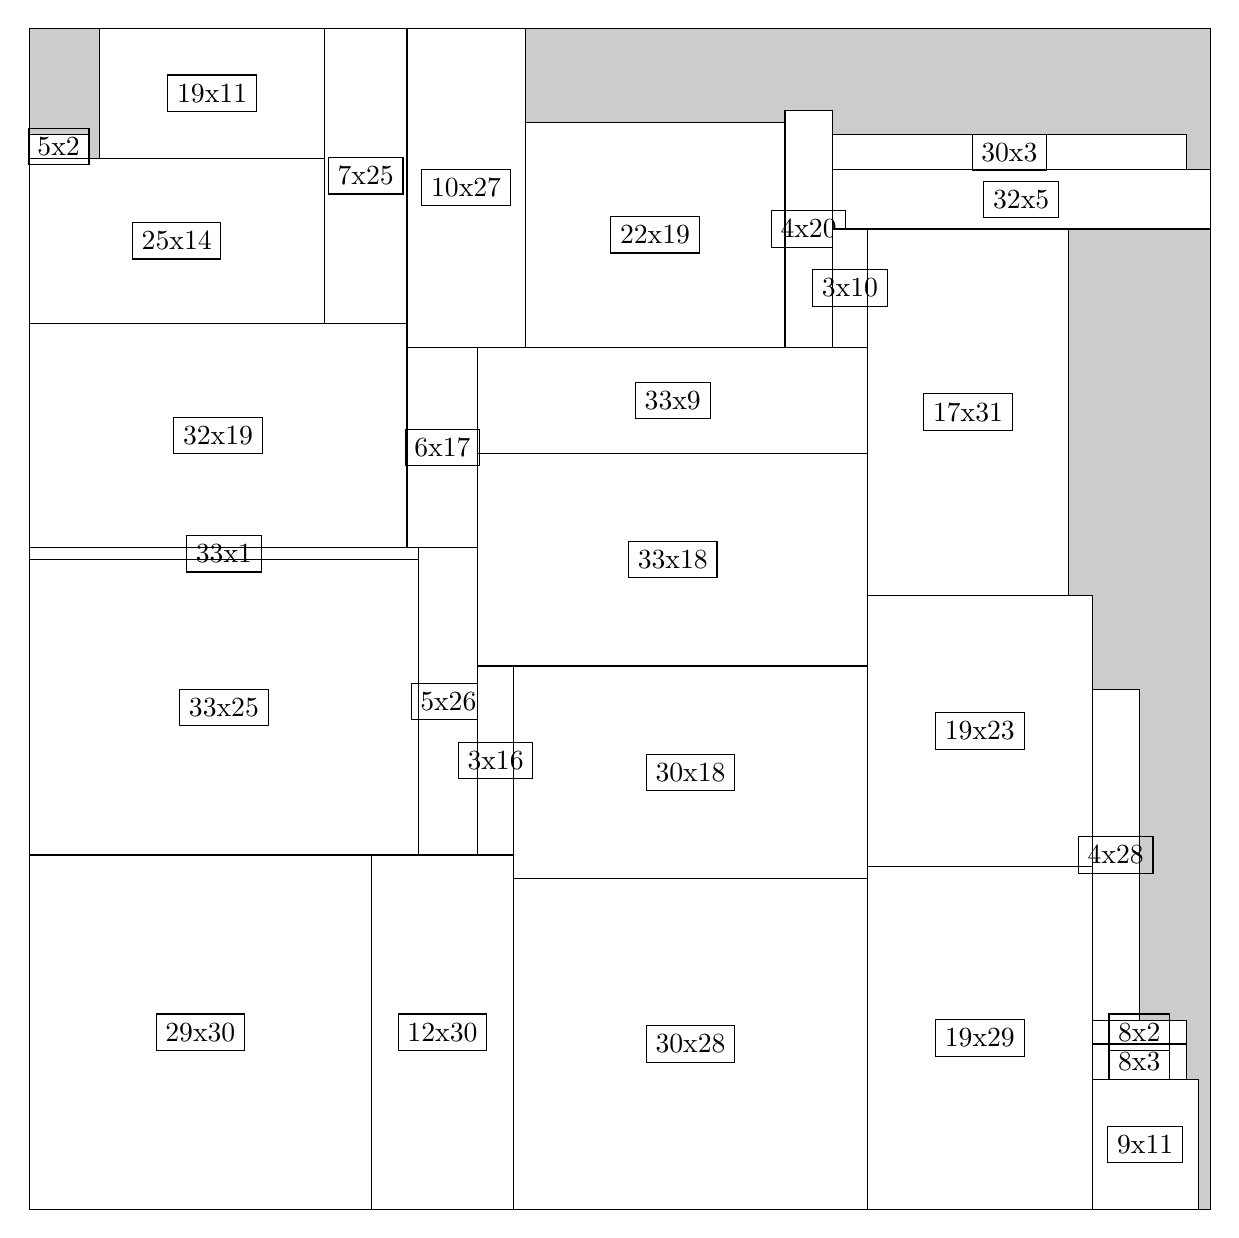
\begin{tikzpicture}[shorten >=1pt,scale=1.0,every node/.style={scale=1.0},->]
\tikzstyle{vertex}=[circle,fill=black!25,minimum size=14pt,inner sep=0pt]
\filldraw[fill=gray!40!white, draw=black] (0,0) rectangle (15.0,15.0);
\foreach \name/\x/\y/\w/\h in {29x30/0.0/0.0/4.35/4.5,30x28/6.1499999999999995/0.0/4.5/4.2,33x25/0.0/4.5/4.95/3.75,32x19/0.0/8.4/4.8/2.85,33x18/5.7/6.8999999999999995/4.95/2.6999999999999997,19x29/10.65/0.0/2.85/4.35,30x18/6.1499999999999995/4.2/4.5/2.6999999999999997,17x31/10.65/7.8/2.55/4.6499999999999995,19x11/0.8999999999999999/13.35/2.85/1.65,22x19/6.3/10.95/3.3/2.85,12x30/4.35/0.0/1.7999999999999998/4.5,25x14/0.0/11.25/3.75/2.1,33x9/5.7/9.6/4.95/1.3499999999999999,10x27/4.8/10.95/1.5/4.05,19x23/10.65/4.35/2.85/3.4499999999999997,7x25/3.75/11.25/1.05/3.75,32x5/10.2/12.45/4.8/0.75,5x26/4.95/4.5/0.75/3.9,4x28/13.5/2.4/0.6/4.2,6x17/4.8/8.4/0.8999999999999999/2.55,9x11/13.5/0.0/1.3499999999999999/1.65,30x3/10.2/13.2/4.5/0.44999999999999996,4x20/9.6/10.95/0.6/3.0,3x16/5.7/4.5/0.44999999999999996/2.4,33x1/0.0/8.25/4.95/0.15,3x10/10.2/10.95/0.44999999999999996/1.5,8x3/13.5/1.65/1.2/0.44999999999999996,8x2/13.5/2.1/1.2/0.3,5x2/0.0/13.35/0.75/0.3}
\filldraw[fill=white!40!white, draw=black] (\x,\y) rectangle node[draw] (\name) {\name} ++(\w,\h);
\end{tikzpicture}


w =29 , h =30 , x =0 , y =0 , v =870
\par
w =30 , h =28 , x =41 , y =0 , v =840
\par
w =33 , h =25 , x =0 , y =30 , v =825
\par
w =32 , h =19 , x =0 , y =56 , v =608
\par
w =33 , h =18 , x =38 , y =46 , v =594
\par
w =19 , h =29 , x =71 , y =0 , v =551
\par
w =30 , h =18 , x =41 , y =28 , v =540
\par
w =17 , h =31 , x =71 , y =52 , v =527
\par
w =19 , h =11 , x =6 , y =89 , v =209
\par
w =22 , h =19 , x =42 , y =73 , v =418
\par
w =12 , h =30 , x =29 , y =0 , v =360
\par
w =25 , h =14 , x =0 , y =75 , v =350
\par
w =33 , h =9 , x =38 , y =64 , v =297
\par
w =10 , h =27 , x =32 , y =73 , v =270
\par
w =19 , h =23 , x =71 , y =29 , v =437
\par
w =7 , h =25 , x =25 , y =75 , v =175
\par
w =32 , h =5 , x =68 , y =83 , v =160
\par
w =5 , h =26 , x =33 , y =30 , v =130
\par
w =4 , h =28 , x =90 , y =16 , v =112
\par
w =6 , h =17 , x =32 , y =56 , v =102
\par
w =9 , h =11 , x =90 , y =0 , v =99
\par
w =30 , h =3 , x =68 , y =88 , v =90
\par
w =4 , h =20 , x =64 , y =73 , v =80
\par
w =3 , h =16 , x =38 , y =30 , v =48
\par
w =33 , h =1 , x =0 , y =55 , v =33
\par
w =3 , h =10 , x =68 , y =73 , v =30
\par
w =8 , h =3 , x =90 , y =11 , v =24
\par
w =8 , h =2 , x =90 , y =14 , v =16
\par
w =5 , h =2 , x =0 , y =89 , v =10
\par
\newpage


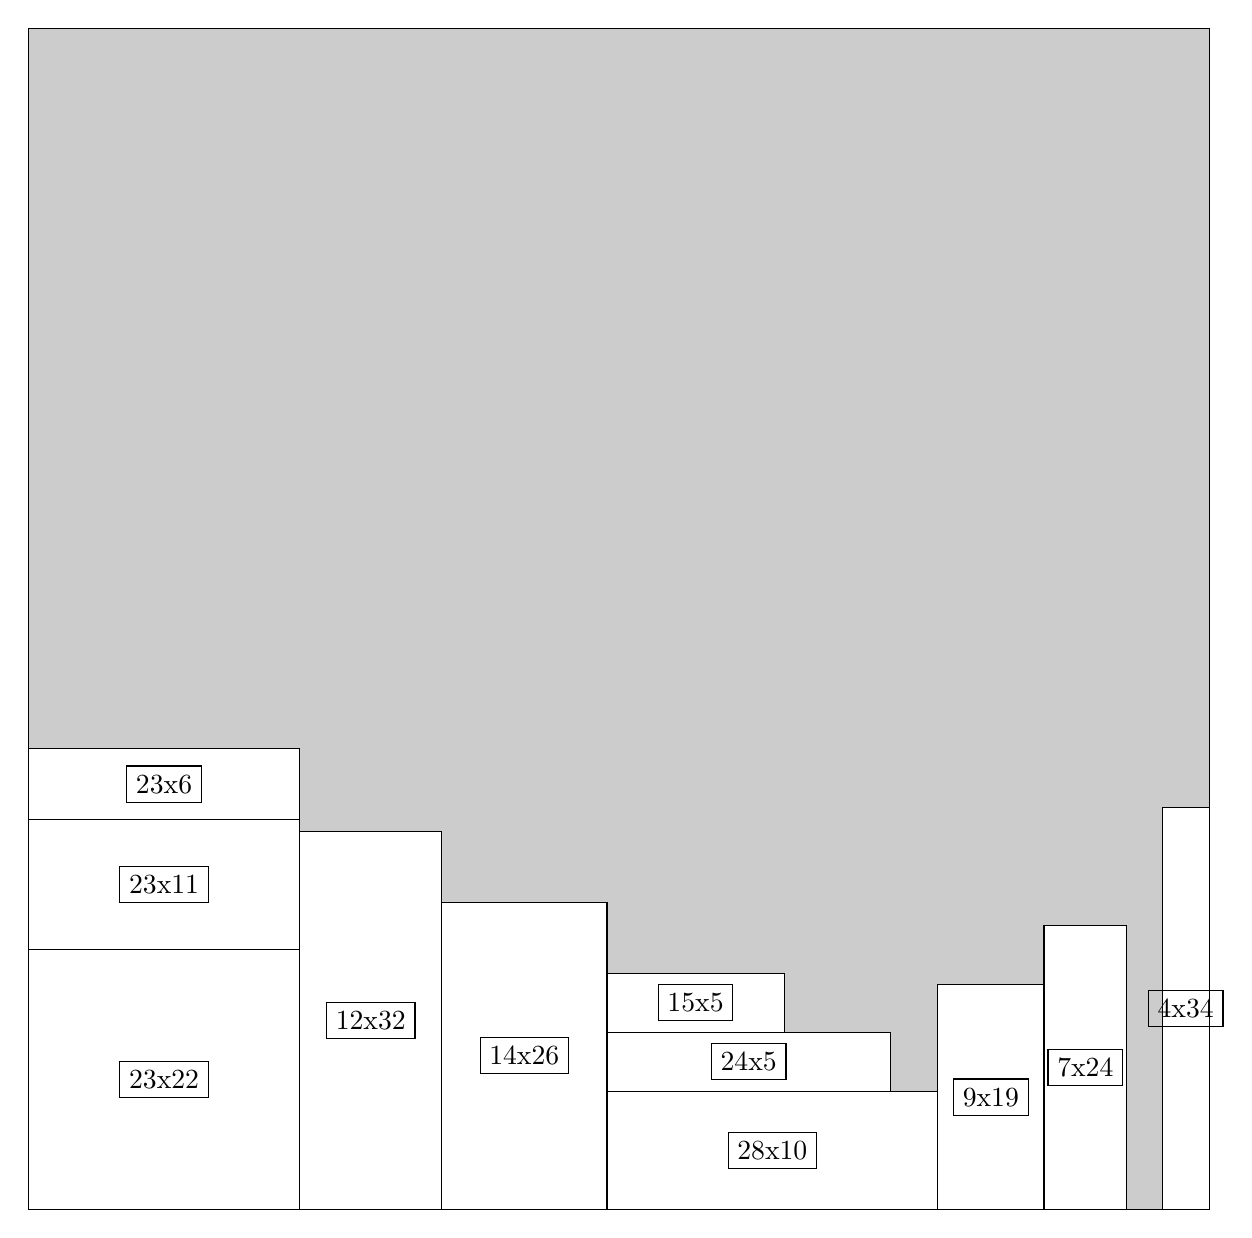
\begin{tikzpicture}[shorten >=1pt,scale=1.0,every node/.style={scale=1.0},->]
\tikzstyle{vertex}=[circle,fill=black!25,minimum size=14pt,inner sep=0pt]
\filldraw[fill=gray!40!white, draw=black] (0,0) rectangle (15.0,15.0);
\foreach \name/\x/\y/\w/\h in {23x22/0.0/0.0/3.4499999999999997/3.3,12x32/3.4499999999999997/0.0/1.7999999999999998/4.8,14x26/5.25/0.0/2.1/3.9,28x10/7.35/0.0/4.2/1.5,23x11/0.0/3.3/3.4499999999999997/1.65,9x19/11.549999999999999/0.0/1.3499999999999999/2.85,7x24/12.9/0.0/1.05/3.5999999999999996,23x6/0.0/4.95/3.4499999999999997/0.8999999999999999,4x34/14.399999999999999/0.0/0.6/5.1,24x5/7.35/1.5/3.5999999999999996/0.75,15x5/7.35/2.25/2.25/0.75}
\filldraw[fill=white!40!white, draw=black] (\x,\y) rectangle node[draw] (\name) {\name} ++(\w,\h);
\end{tikzpicture}


w =23 , h =22 , x =0 , y =0 , v =506
\par
w =12 , h =32 , x =23 , y =0 , v =384
\par
w =14 , h =26 , x =35 , y =0 , v =364
\par
w =28 , h =10 , x =49 , y =0 , v =280
\par
w =23 , h =11 , x =0 , y =22 , v =253
\par
w =9 , h =19 , x =77 , y =0 , v =171
\par
w =7 , h =24 , x =86 , y =0 , v =168
\par
w =23 , h =6 , x =0 , y =33 , v =138
\par
w =4 , h =34 , x =96 , y =0 , v =136
\par
w =24 , h =5 , x =49 , y =10 , v =120
\par
w =15 , h =5 , x =49 , y =15 , v =75
\par
\newpage


\end{document}